
% ==================================================
%	Theorie
% ==================================================

\section{Theorie}

Die Tomographie ist ein bildgebendes Verfahren, also eine Technik, die
Verteilung physikalischer Eigenschaften, wie z.B.~den Absorptionskoeffizienten,
eines Objektes zu visualisieren. Durch verschiedene Querschnittsbilder kann so
die Struktur des Objektes ermittelt werden. In diesem Versuch wird zur
Untersuchung der Struktur der Würfel $\gamma$-Strahlung eines
\Cs~-Strahlers verwandt.
Der Würfel wird nun aus einer Richtung bestrahlt, wobei die Strahlung damit in
seiner Intensität geschwächt wird.
Wie stark die Intensität geschwächt wird, hängt von
den in dem Würfel vorkommenden Materialien ab. Dieser Vorgang wird von
verschiedenen Richtungen wiederholt.
So kann theoretisch ein dreidimensionales Abbild des
Würfels erstellt werden kann. Die in diesem Versuch verwandten Würfel bestehen
aus $3\times 3 \times 3$ Elementarwürfel, wobei nur die mittlere Ebene
ausgemessen wird.~\cite{AP} Die Tomographie baut also auf das Verständnis der
Wechselwirkung von $\gamma$-Strahlung mit Materie auf.
Diese sollen nun kurz beschrieben werden.

% ==================================================
% 	Erzeugung von Gamma-Strahlung
% ==================================================
\subsection{Erzeugung von $\gamma$-Strahlung}
\label{sub:erzeugung_von_gamma_strahlung}

Wie eingangs erwähnt wird in diesem Versuch zur Erzeugung von
$\gamma$-Strahlung das radioaktive Isotop \Cs~verwandt.
Das Zerfallsschema von \Cs~ist in Abbildung~\ref{fig:Cs}
dargestellt.
Hieran ist zu erkennen, dass \Cs~mit einer Halbwertszeit von 30.08 Jahren
zu fast \SI{100}{\percent} durch einen
$\beta^-$-Zerfall in einen angeregten Zustand von \Ba~zerfällt.
Dieser angeregte Zustand zerfällt schließlich unter Aussendung von
$\gamma$-Strahlung in den Grundzustand.
Hierbei ergibt sich eine $\gamma$-Linie mit der Energie \SI{662}{\keV}.
Diese Linie wird zur Bestimmung der Struktur der Würfel
verwandt.
\begin{figure}[t]
  \centering
  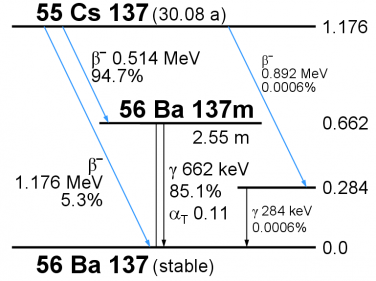
\includegraphics[scale=0.6]{bilder/376px-Cs137keV.png}
  \caption{Darstellung des Zerfallsschema von \Cs~.\cite{Cs137}}
\label{fig:Cs}
\end{figure}

\newpage
% ==================================================
% 	Wechselwirkung Gamma Strahlung
% ==================================================
\subsection{Wechselwirkung von $\gamma$-Strahlung mit Materie}
\label{sub:wechselwirkung_von_gamma_strahlung_mit_materie}

Die wesentlichen Effekte, welche bei der Wechselwirkung von $\gamma$-Strahlung
mit Materie auftrete sind
\begin{enumerate}
  \item Photo-Effekt
  \item Compton-Streuung
  \item Paar-Produktion~.
\end{enumerate}
Bei dem Photo-Effekt wird ein Photon von einem Elektron einer Atomhülle
absorbiert, wobei anschließend das Elektron aus der Atomhülle gelöst wird.
Der Compton-Effekt beschreibt hingegen die Streuung eines Photons mit einem
freien Elektron. In der Materie sind die Elektronen zwar gebunden, aber bei
einer hohen Photonenenergie im Vergleich zur Bindungsenergie kann die
Bindungsenergie vernachlässigt werden. So kann die Bindungsenergie in der
Größenordnung der Grundzustandsenergie des Wasserstoffatoms mit \SI{13.6}{\eV}
abgeschätzt werden. Somit ist dies im Vergleich mit der $\gamma$-Linie mit
$\sim \SI{660}{\keV}$ vernachlässigbar und die Elektronen können als frei
betrachtet werden.
Die Paar-Produktion ist dagegen ein Prozess in dem ein Photon in ein Elektron
und ein Positron übergeht. Aufgrund der Impulserhaltung kann dies nur durch
Anwesenheit eines dritten Körpers geschehen. Zudem muss die Energie des Photons
mindestens zwei mal die Ruheenergie des Elektrons bzw.~des Positrons betragen.
Mit der Ruheenergie von $\sim \SI{0.5}{MeV}$ muss das Photon ca. \SI{1}{\MeV}
betragen. Die $\gamma$-Linie von \Cs~liegt aber darunter,
sodass die Paar-Produktion keine Rolle spielt.
Somit sind die wesentliche Effekte in diesem Versuch der Photo-Effekt und
der Compton-Effekt.

% ==================================================
% Bestimmung der Absorptionskoeffizienten
% ==================================================
\subsection{Bestimmung der Absorptionskoeffizienten}
\label{sub:bestimmung_der_absorptionskoeffizienten}

Um die Struktur der Würfel zu bestimmen wird der Würfel nun mit
$\gamma$-Strahlung der \Cs-Quelle bestrahlt.
Diese Strahlung durchdringt den Würfel. Die Intensität der Strahlung nach
Durchdringen des Würfels kann ausgedrückt werden durch
\begin{equation}
  N = I_0\ \e^{-\sum \mu_i d_i}~,
  \label{eq:Intensität}
\end{equation}
wobei $\mu_i$ die Absorptionskoeffizienten und $d_i$ die Wegstrecken, welche
die Strahlung durch die Elementarwürfel läuft, sind. Bei bekannter
Eingangsintensität $I_0$ und bekannten Eingangsintensitäten $N_j$ der $j$-ten
Projektion, kann Gleichung~\eqref{eq:Intensität} umgestellt werden zu
\begin{equation}
  \sum \mu_i d_i = \ln(\frac{I_0}{N_j})~.
  \label{eq:Intensitaet_umgestellt}
\end{equation}
Dies stellt ein lineares Gleichungssystem dar, sodass durch Ausmessen
verschiedener Projektionen die Absorptionskoeffizienten bestimmt werden können.
Die Gleichung~\eqref{eq:Intensitaet_umgestellt} kann für $m$ Messungen
zweckmäßig auch geschrieben werden als
\begin{equation}
  \begin{gathered}
  A\ \vec{\mu} = \vec{I} \\
  \vec{\mu} = \qty(\mu_1, \dotsc, \mu_9)~,
  \qquad \vec{I} = \qty(I_1, \dotsc, I_m)~,
  \qquad I_j = \ln(\frac{I_0}{N_j})~.
  \end{gathered}
\end{equation}
Hierbei beschreibt die Matrix $A$ die Würfelgeometrie. Um die Messgenauigkeit
zu erhöhen, werden mehr Projektionen als Elementarwürfel gemessen, sodass das
Gleichungssystem überbestimmt ist. Mit Hilfe der Methode der kleinsten Quadrate
können schließlich die Absorptionskoeffizienten bestimmt werden.
In der Methode der kleinste Quadrate geht es darum, die quadratischen
Abweichungen (Residuen) eines Modells zu den Daten zu
minimieren.\cite{blobel1998statistische}
Das Modell ist hier linear und durch $f(\vec{\mu}) = A \vec{\mu}$ mit dem
Parametern $\vec{\mu}$ gegeben.  Das Quadrat der Residuen lautet
\begin{equation}
  \vec{r}^\top \vec{r} =
  {\qty(\vec{I} - A\vec{\mu})}^\top \qty(\vec{I} - A\vec{\mu})~.
\end{equation}
Leitet man diese Gleichung nach den $\mu_i$ ab und setzt das Ergebnis gleich
null, so folgt die sogenannte Normalengleichung
\begin{equation}
  \qty(A^\top A) \vec{\mu} = \qty(A^\top \vec{I})~,
  \label{eq:normalengleichung_ohne_fehler}
\end{equation}
woraus die Absorptionskoeffizienten entsprechend
\begin{equation}
  \vec{\mu} = {\qty(A^\top A)}^{-1} A^\top \vec{I}
\end{equation}
bestimmt werden können. Diese Betrachtung gilt allerdings nur für den Fall,
dass jede Einzelmessung $I_i$ die selbe Standardabweichung hat.
In diesem Versuch hat jedoch jede Einzelmessung einen anderen Fehler.
Hierfür lautet die umgestellte Normalengleichung nun
\begin{equation}
  \vec{\mu} = {\qty(A^\top W A)}^{-1} A^\top W \vec{I}
  \label{eq:mu}
\end{equation}
mit der Gewichtsmatrix
\begin{equation}
  W(\vec{\mu}) =
  \begin{pmatrix}
    1\ /\ \sigma_1^2 & 0 & 0 & \dotsc & 0 \\
    0 & 1\ / \ \sigma_2^2 & 0 & \dotsc & 0 \\
    & \dotsc & & \\
    & \dotsc & & \\
    0 & 0 & 0 & \dotsc & 1\ /\ \sigma_m^2
  \end{pmatrix}~.
  \label{eq:gewichtsmatrix}
\end{equation}
Die Varianzen der Absorptionskoeffizienten ergeben sich aus den
Diagonaleinträgen der Varianzmatrix
\begin{equation}
  V(\vec{\mu}) = {\qty(A^\top W A)}^{-1}~.
  \label{eq:varianzmatrix}
\end{equation}

